\documentclass[11pt]{article}
\usepackage{amsmath, amssymb, amsthm}
\usepackage{geometry}
\usepackage{graphicx}
\usepackage{subcaption} % make sure this is here
\geometry{margin=1in}
\setlength\parindent{0pt}
\title{Foundations of Machine Learning -- Lecture 6 Notes}
\author{}
\date{}

\begin{document}
\maketitle

\section*{Clustering}

Dimensionality Reduction
\[
	X \in \mathbb{R}^{Nxd} \rightarrow Z \in \mathbb{R}^{Nxm}, m << d
\]

Clustering
\[
	X \in \mathbb{R}^{Nxd} \rightarrow Z \in \mathbb{R}^{kxd}, k << N
\]

The main idea with clustering is to reduce the number of data points within a particular set by grouping together similar instances.

\begin{figure}[h]
	\centering
	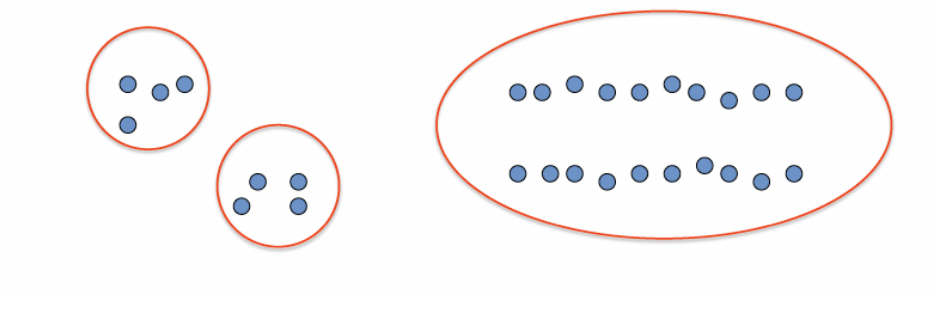
\includegraphics[width=0.35\textwidth]{../imgs/clust-exam.png} % 
	\caption{Example ROC Curve}
\end{figure}

To find out weather points are similar we use a distance formula.
\[
	dist(x^{(i)}, x^{(j)})
\]

\section*{K-Means Clustering}

This is an iterative algorithm for clustering
\medskip

Input: Data ${x^{(i)},\dots,x^{(N)} \in \mathbb{R}^d}$
\medskip

Output: Centroids ${u^{(i)},\dots,x^{(K)} \in \mathbb{R}^d}$
\medskip

Process:
\begin{enumerate}
	\item Initilaize with K random centroids
	\item Repeat until convergence
	      \begin{itemize}
		      \item Assign a cluster to every sample $x^{(i)} \Rightarrow c^{(i)} = \arg\min_k dist(x^{(i)}, u^{(k)})$
		      \item Update centroids according to clusters: \[
			            \mu^{(k)} =
			            \frac{\displaystyle \sum_{i=1}^{N} \mathbf{1}_{c_i = k} \, x^{(i)}}
			            {\displaystyle \sum_{i=1}^{N} \mathbf{1}_{c_i = k}}
		            \]

	      \end{itemize}
\end{enumerate}

\pagebreak

\begin{figure}[h]
    \centering
    \begin{subfigure}[b]{0.24\textwidth}
        \centering
        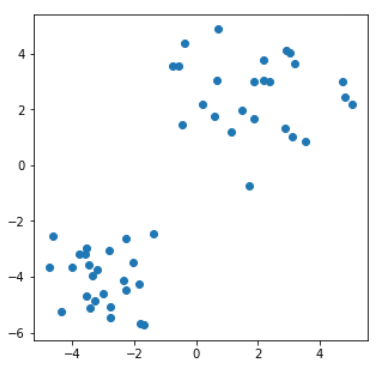
\includegraphics[width=\linewidth]{../imgs/knn-proc-1.png}
        \caption{Step 1}
    \end{subfigure}
    \begin{subfigure}[b]{0.24\textwidth}
        \centering
        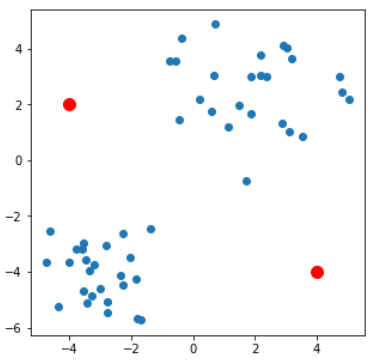
\includegraphics[width=\linewidth]{../imgs/knn-proc-2.png}
        \caption{Step 2}
    \end{subfigure}
    \begin{subfigure}[b]{0.24\textwidth}
        \centering
        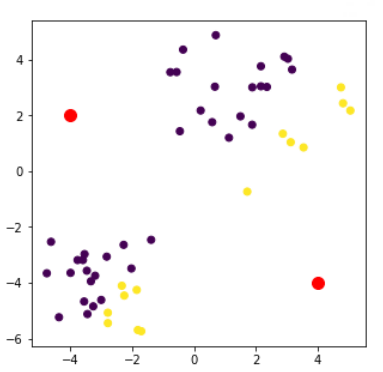
\includegraphics[width=\linewidth]{../imgs/knn-proc-3.png}
        \caption{Step 3}
    \end{subfigure}
    \begin{subfigure}[b]{0.24\textwidth}
        \centering
        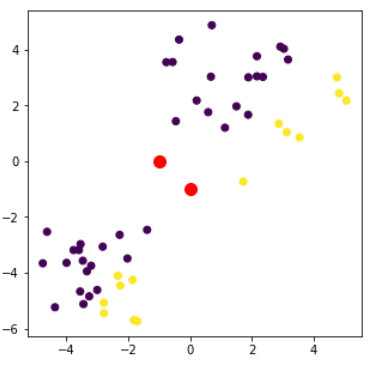
\includegraphics[width=\linewidth]{../imgs/knn-proc-4.png}
        \caption{Step 4}
    \end{subfigure}
    \caption{KNN process}
\end{figure}




This is \textbf{guaranteed} to converge with a finate amount of steps
\medskip

Time complexity:
\begin{itemize}
	\item Assign data points to closes centroid: $O(KN)$
	\item Change the cluster center to the average of its assigned points $O(N)$
\end{itemize}

\subsection*{Derivation}

We want to find $Z = [u^{(i)}, \dots, u^{(K)}]^T \in \mathbb{R}^{k \times d}$ such that it minimizes teh within cluster variance of our dataset X.

To calculate the within cluster variance we find:
\[
	\sum_{k=1}^{K} \sigma_k^2
	=
	\sum_{k=1}^{K} \sum_{i} \left\| x^{(i)} - \mu^{(k)} \right\|^2 \quad s.t \; c^{(i)} = k
\]

We define the \textbf{cluster assignments} as:
\[
	C = [c(1), \dots, c(n)], \qquad c(i) \in \{1, \dots, K\}.
\]

Here, $c(i)$ denotes the index of the cluster to which data point $x^{(i)}$ is assigned.

\medskip

We define the \textbf{cluster centers (centroids)} as:
\[
	Z = [\mu^{(1)}, \dots, \mu^{(K)}]^T \in \mathbb{R}^{K \times d}.
\]

Each $\mu^{(k)} \in \mathbb{R}^d$ is the centroid of cluster $k$, given by the mean of all data points assigned to that cluster.

\paragraph{Original optimization problem.}
\[
	\min_{C, Z} \quad \sum_{k=1}^{K} \sum_{i \,:\, c(i)=k} \left\| x^{(i)} - \mu^{(k)} \right\|^2
\]

This is computationally intractable and we can break this up into 2 subproblems instead.

\paragraph{2 subproblem optimization approach.}

\begin{itemize}
	\item \textbf{For fixed } $Z = [\mu^{(1)}, \dots, \mu^{(K)}]^T$, \textbf{optimize } $C$:
	      \[
		      \min_{C} \quad \sum_{i=1}^{N} \left\| x^{(i)} - \mu^{(c(i))} \right\|^2
	      \]

	\item \textbf{For fixed } $C$, \textbf{optimize } $Z$:
	      \[
		      \min_{Z} \quad \sum_{k=1}^{K} \sum_{i} \left\| x^{(i)} - \mu^{(k)} \right\|^2\quad s.t \; c^{(i)} = k
	      \]

\end{itemize}

\begin{figure}[h]
	\centering
	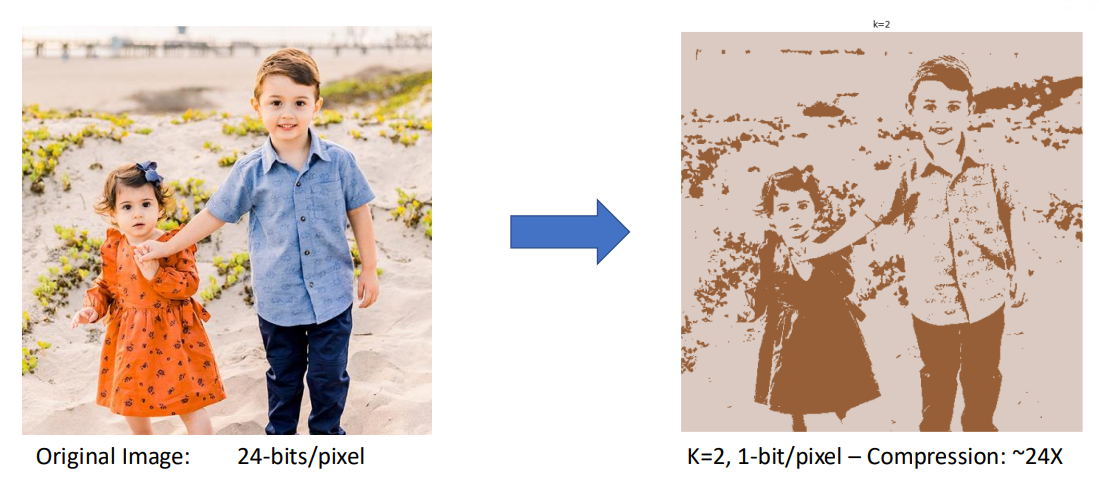
\includegraphics[width=0.4\textwidth]{../imgs/img-cluster-ex.png}
	\caption{K-Means: Image Compression}
\end{figure}

\subsection*{Issues with K-Means}
K-Means is a \textbf{non-convex} optimization problem, so the algorithm typically converges to a \textbf{local minimum}, not necessarily the global minimum. Consequently,
\begin{itemize}
    \item The same dataset may yield different clustering results under different initializations, and
    \item Initialization plays a critical role in the final outcome.
\end{itemize}

\begin{figure}[h]
	\centering
	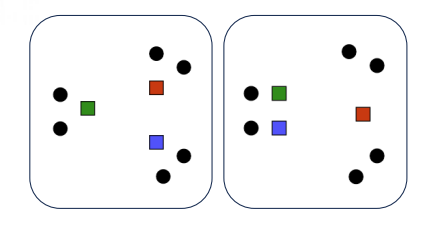
\includegraphics[width=0.35\textwidth]{../imgs/kissue.png}  
	\caption{Different clusters on same input}
\end{figure}

\pagebreak

\subsection*{Choice of distance matters!}

\begin{figure}[h]
	\centering
	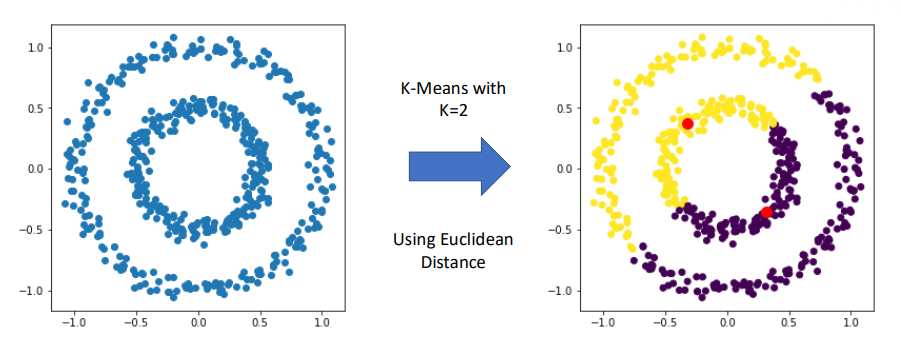
\includegraphics[width=0.35\textwidth]{../imgs/kmeans-euc.png}  
	\caption{K-Means with euclidian distance}
\end{figure}

\begin{figure}[h]
	\centering
	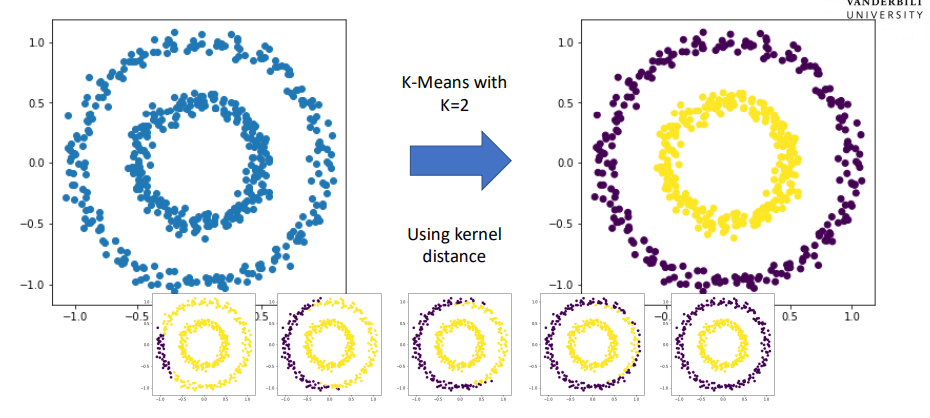
\includegraphics[width=0.35\textwidth]{../imgs/kmeans-ker.png} 
	\caption{K-Means with kernel distance}
\end{figure}



\subsection*{How to find the right K}

\paragraph*{The Elbow Method}
Calculate the Within-Cluster-Sum of Squared Errors (WSS) for different values of k. In the plot of WSS versus-k, the optimal k value is visible as an elbow.

\paragraph*{The Silhouette Method}

\[
s(o) = \frac{b(o) - a(o)}{\max\{a(o),\, b(o)\}}
\]

\noindent where:
\begin{itemize}
    \item $s(o)$ is the silhouette coefficient of data point $o$,
    \item $a(o)$ is the \textit{average distance} between $o$ and all other data points in the cluster to which $o$ belongs,
    \item $b(o)$ is the \textit{minimum average distance} from $o$ to all clusters to which $o$ does not belong.
\end{itemize}

The silhouette coefficient measures how well a data point fits within its assigned cluster and how far it is from neighboring clusters.

\[
-1 \leq s(o) \leq 1
\]
\begin{itemize}
    \item $s(o) = 1$ indicates that the data point is well-clustered,
    \item $s(o) = -1$ indicates that the data point is misclassified,
    \item $s(o) = 0$ indicates that the data point lies on a cluster boundary.
\end{itemize}

We want to calculate $s(o)$ for different k values and choose the result with the highest score.

\end{document}



